%
% File acl2016.tex
%
%% Based on the style files for ACL-2015, with some improvements
%%  taken from the NAACL-2016 style
%% Based on the style files for ACL-2014, which were, in turn,
%% Based on the style files for ACL-2013, which were, in turn,
%% Based on the style files for ACL-2012, which were, in turn,
%% based on the style files for ACL-2011, which were, in turn, 
%% based on the style files for ACL-2010, which were, in turn, 
%% based on the style files for ACL-IJCNLP-2009, which were, in turn,
%% based on the style files for EACL-2009 and IJCNLP-2008...

%% Based on the style files for EACL 2006 by 
%%e.agirre@ehu.es or Sergi.Balari@uab.es
%% and that of ACL 08 by Joakim Nivre and Noah Smith

\documentclass[11pt]{article}
\usepackage{acl2016}
\usepackage{times}
\usepackage{url}
\usepackage{latexsym}
\usepackage{graphicx}
\usepackage{amsmath}
\usepackage{float}
\usepackage{floatrow}


%\aclfinalcopy % Uncomment this line for the final submission
%\def\aclpaperid{***} %  Enter the acl Paper ID here

%\setlength\titlebox{5cm}
% You can expand the titlebox if you need extra space
% to show all the authors. Please do not make the titlebox
% smaller than 5cm (the original size); we will check this
% in the camera-ready version and ask you to change it back.

\newcommand\BibTeX{B{\sc ib}\TeX}

\title{Character Identification on Multiparty Dialogue based on End-to-End Neural Coreference Resolution}

\author
{
   Pu-Chin Chen
  {\tt \{puchinchen@ucla.edu\}} \\
  Aoxuan Li 
  {\tt \{a811278305@gmail.com\}} \\
  Yutian Zhang
  {\tt \{yutianzh0527@gmail.com\}} \\
  Xin Liu
  {\tt \{xinliu627@ucla.edu\}} \\
}

\date{}

\begin{document}
\maketitle
\begin{abstract}
  Coreference resolution and entity linking are two important research topics in NLP, gaining growing attentions over years. In this project, we combined these two tasks together to accomplish a more complicated task, which is identifying the characters in multiparty dialoagues. Different from previous traditional methods of coreference resolution, a state-of-the-art end-to-end model is adoptd, which significantly outpeforms other previous work.In addition, our entity-linking model is based on CNN instead of knowledge databases. Finally,we evaluated our models using the scripts from real TV shows.The results of coreference resolution are satisfactory, but the performance of entity linking does not live up to our expections.We analyzed the possible underlying reasons, which pointing out the research direction in future work.
\end{abstract}

\section{Introduction}

Our main goal is to accomplish a shared task in SemEval 2018 - Task 4: Character Identification on Multiparty Dialogues. This tasks requires us to build a system which can identify different mentions in multiparty dialogues as corresponding characters in the show.This task is rather challenging, for cross-document entity resolution is imperative for identifying such mentions as real characters.

Literally, the character identification problem is tackled as a coreference resolution task with a further step on entity linking.In terms of this task, the baseline model generates mentions from a coreference system, and then each coreference chain is linked to a specific character identity. Both parts are implemented with agglomerative convolutional neural network in previous system \cite{Robust,Character}.Alternatively, we intend to use Bidirectional-LSTM with attention mechanism to address the same problem, which proves to have a satisfying performance in many NLP tasks. In our project, we apply the end-to-end neural coreference resolution model introduced by Lee and He, etc.\cite{2017arXiv170707045L}. After obtaining the predicted clusters of mentions by the end-to-end coreference system, we choose the same algorithm of entity-linking as the one Chen proposed in his paper \cite{Robust}.

\section{Related Works}
\subsection{Coreference resolution}
The area of coreference resolution has resorted to the techniques of machine learning for many years. Still, the learning problem is challenging and, until very recently, hand-engineered systems built on top of automatically produced parse trees \cite{Raghunathan:2010:MSC:1870658.1870706} outperformed all learning approaches.\cite{Durrett2013EasyVA} showed that highly lexical learning approaches reverse this trend, and more recent neural models\cite{2016arXiv160403035W,2016arXiv160908667C,2016arXiv160601323C} have achieved noticeable performance gains. However, all of the aforementioned models still use parsers for head features and include highly engineered mention proposal algorithms.Such pipelined systems suffer from two major drawbacks. First, parsing mistakes can introduce cascading errors. Second, many hand-engineered rules do not generalize ideally to new languages or domains.  

\subsection{Entity Linking}

Entity linking has traditionally relied heavily on knowledge databases, most notably, Wikipedia, for entities 
\cite{Mihalcea:2007:WLD:1321440.1321475,2016arXiv160400734F}.Although we do not make use of knowledge bases, our task is closely aligned to entity linking. Recent advances in entity linking are also applicable to our task since \cite{2016arXiv160400734F} use CNN to capture semantic similarity between a mention and an entity by comparing context of the mention with the description of the entity. This work justifies our usage of deep learning for character identification.

As indicated by the Dialogue State Tracking Challenges hosted by Microsoft  \cite{Fourth}, the dialogue tracking is an expanding task. The fact that an ongoing conversation can be dynamically tracked \cite{henderson-thomson-young:2013:SIGDIAL}is exciting and applicable to our task because the state of a conversation may yield significant hints for entity linking and coreference resolution. Speaker identification, a task similar to character identification, has already shown some success with partial dialogue tracking by dynamically identifying speakers at each turn in a dialogue using conditional random field models.

\section{End-to-End Coreference Resolution}

\subsection{Inroduction}
Recent coreference models usually rely on syntactic parsers. However, the end-to-end coreference resolution directly consider all the spans up to a maximum length in the document as potential mentions,  compute the probability of possible ancestors (previous span) for each span, and directly optimizes the marginal likelihood of antecedent spans from gold coreference clusters.

Since the number of potential mentions is very large, it is impractical to score all span pairs. So this model uses unary mention scores to prune the space of pairs of spans(spans and antecedents), which significantly reduce the pairwise computations.

\subsection{Model}

\begin{figure}[h]
                
 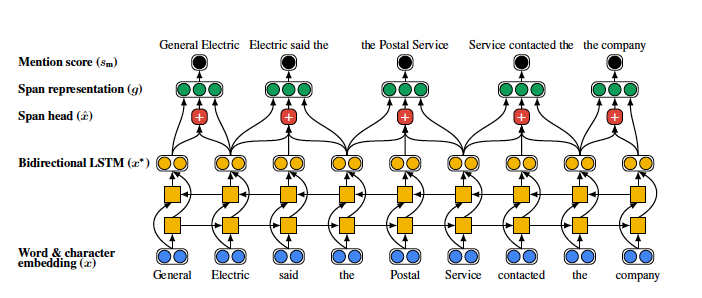
\includegraphics[width=0.5\textwidth]{02.jpg}
 \caption{First step of the model}
                
\end{figure}

First step:  computes embedding representations of spans for scoring potential entity mentions.
A  bidirectional LSTM is used to encode the lexical information of both the inside and outside of each span. The model also includes a head-finding attention mechanism over words in each span to model head words.
We use score to prune the spans, leaving only a manageable number of high-score spans for further steps.

\begin{figure}[h]                
 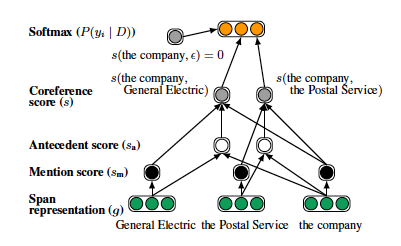
\includegraphics[width=0.5\textwidth]{03.jpg}
 \caption{Second step of the model}             
\end{figure}

Second step: compute antecedent scores for each pair of spans. And then sum the mention scores of both spans and their pairwise antecedent score as the final coreference score of this pair of spans.
The antecedent scoring function includes explicit element-wise similarity of each span pair and a learned 20-dimensional feature vector which encoding all features like speaker genre, span distance, mention width.

Learning: We optimize the marginal log-likelihood of all correct antecedents implied by the gold clustering:

\begin{equation}
log\prod^{N}_{i=1}\sum_{\widehat{y}\in Y(i)\cap \text{GOLD}(i)}P(\widehat{y})
\end{equation}


where GOLD(i) is the set of spans in the gold cluster containing span i. If span i does not belong to a gold cluster or all gold antecedents have been pruned, GOLD(i) = \{$\varepsilon $\}.

\subsection{Ablations}
To show whether each component in our model is actually important, we ablate various parts of the architecture and report the average F1 on these experiments. We conducted one complete experiment and two ablation experiments, no heads and no features. In our dataset, the width of mention is always one or two word, the head-finding attention mechanism for each span seems to be useless, so we select no head ablation to verify this guess.  And we also want to show the significance of feature encoding.


\section{Entity Linking}

\subsection{Introduction}
Once the coreference resolution system is built and trained, we can predict co-references represented by clusters for each scene document. The next step should be making predictions from clusters to TV show character id. We model this process as an entity linking task. This section describes our entity linking model that takes the mention embeddings and the mention-pair embeddings generated by ACNN and classifies each mention to one of the character labels.

\subsection{Model}
\begin{figure}[h]                
 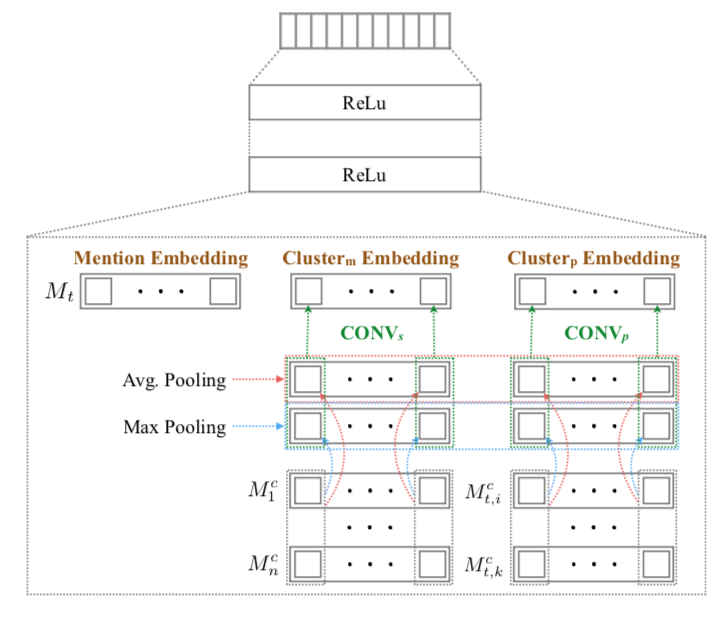
\includegraphics[width=0.5\textwidth]{05.jpg}
 \caption{Character identification model}             
\end{figure}

We prepare three embeddings generated by mentions which are predicted by precious co-reference system. The first embedding is mention embedding; the second is embedding of the cluster including the mention; the third is generated by mention-pair embedding, which pairs the mention with reaming mention in the same cluster. Here are the formal formula:
\begin{eqnarray}
\mathbf{R}_s(C_m) = [\mathbf{r}_s(m_1),\mathbf{r}_s(m_1),...,\mathbf{r}_s(m_{|C_m|})]\\
\mathbf{R}_p(C_m,m) = [\mathbf{r}_p(m_i,m)|m_i \neq m]
\end{eqnarray}



In order to fix the input tensor size of both cluster embedding and mention-pair embedding, we perform avg-pooling and max-pooling for both embeddings. Then each of pooling layers is passed to a convolutional layer. Finally, we concat the mention embedding, cluster CNN embedding and mention-pair CNN embedding.

\begin{equation}
\mathbf{r}_s(C_m) = \textrm{CONV}_s(\begin{bmatrix}
\text{avg\_pool}(\mathbf{R}_s(C_m))\\
\text{max\_pool}(\mathbf{R}_s(C_m))
\end{bmatrix}
\end{equation}


\begin{equation}
\mathbf{r}_p(C_m,m) = \textrm{CONV}_p(\begin{bmatrix}
\text{avg\_pool}(\mathbf{R}_s(C_m,m))\\
\text{max\_pool}(\mathbf{R}_s(C_m,m))
\end{bmatrix}
\end{equation}


After concatenation, we feed them into a feed-forward neural network with two hidden layers. Final output is a softmax with the idmention of entity id number in Friends TV show.

\subsection{Implementation}
Our training data has 374 documents, which contains totally 13280 gold mentions that have gold entity label. Firstly, we need to get gold clusters and generate three embeddings, i.e. mention, cluster and mention pair embeddings. Since all gold clusters are labeled with entity ids, we can flat clusters to mentions while computing three embeddings. We can easily get mention embeddings from the pretrained coref model.


\section{Dataset and Evalution Metrics}
\subsection{Data Description}
The data comes from the scripts of the first two seasons of TV show Friends, which are already annotated for this task. Specifically, each season consists of episodes, and each episode is comprised of scenes.Furthermore, each scene is segmented into sentences.All datasets follow the CoNLL 2012 Shared Task data format. Each sentence is delimited by a new line and each column indicates the information regarding the word or the punctuation.
\begin{table*}[]
\centering
\label{my-label}
\begin{tabular}{|l|l|l|l|l|l|l|l|l|l|}
\hline
        & \multicolumn{3}{l|}{No Features} & \multicolumn{3}{l|}{No Heads} & \multicolumn{3}{l|}{Normal}   \\ \hline
        & F1       & R   & P  & F1      & R  & P & F1      & R  & P \\ \hline
MUC     & 79.14\%  & 76.98\%  & 81.42\%    & 80.90\% & 80.38\% & 81.43\%   & 80.84\% & 81.64\% & 80.71\%   \\ \hline
B\textsuperscript{3}      & 60.68\%  & 55.22\%  & 67.34\%    & 64.38\% & 62.54\% & 66.34\%   & 65.39\% & 68.89\% & 62.23\%   \\ \hline
CEAF\textsubscript{e} & 48.47\%  & 48.21\%  & 48.43\%    & 52.89\% & 50.54\% & 55.48\%   & 51.80\% & 53.51\% & 50.20\%   \\ \hline
AVG     & 62.76\%  & 60.14\%  & 65.73\%    & 66.06\% & 64.49\% & 67.75\%   & 66.02\% & 68.02\% & 64.17\%   \\ \hline
\end{tabular}
\caption{Results on No Features, No Heads, and Normal}
\end{table*}
\subsection{Data Split}
Considering the amount of total data is not so sufficient, we simply split them into two datasets for different purposes, training and evaluation sets. The exact raito of our training set to our evaluation set is 4:1. The evaluation set contains seventy-four scenes in \textit{Friends}.

\subsection{Coreference Evaluation Metrics}
The coreference results are evaluated with three metrics apropos coreference resolution:MUC, $B^{3}$,and $CEAF_e$.The precision, recall and F1 score of each metric approach are calculate separately and then the averages of them are obtained, which are utilized to compare against each other.

\textbf{MUC}\\
MUC(Vilain et al.,1995) concerns the number of pairwise links needed to be inserted or removed to map system responses to gold keys.The number of links shared by  system and gold are calculated. In addition,minimum numbers of links needed to describe coreference chains of the system and gold are computed as well.

\textbf{B\textsuperscript{3}} \\
Rather than evaluating coreference chains merely on their links,$B^{3}$(Bagga and Baldwin,1998) metric computes precision and recall on a mention level.System performance is evaluated by the average of all mentions scores.


\textbf{CEAF\textsubscript{e}} \\
$CEAF_e$(Luo,2005) metric further clarifies the downside of $B^{3}$, in which entites can be used more than once during evaluation. Consequently, both multiple coreference chains of the same entity and chains with mentions of multiple entities are not penalized.To mitigate the aforementioned problem, $CEAF_e$ evaluates exclusively on the best one-to-one mapping between the system’s and gold’s entities.


\section{Results and Analysis}


\subsection{Coreference Resolution Results}
We conducted one complete experiment and two ablation experiments, no heads and no features. The result of no features is shown in Table 1.



\subsection{Entity Linking Results}
We only got about 20\% accuracy on character identification prediction, addressing that simply using combination of mention embeddings generated from coreference system is weak for predcting entity ids. It fails to contain cluster information even though the coreference system does be trained to optimize the clustering accuracy. 

Another issue is that our models actually overfit. In the beginning, we used the ACNN model and overfit quite easily. Then we tried to reduce model complexities by only using one layer feed-forward neural network on mention embeddings, getting rid of cluster embedding and mention pair embedding. However, the preditcion precision is still low. This problem is arisen from two reasons. Firstly, this dataset is too small to use very complex model like deep neural networks. Secondly, consider our model, mention embeddings are extracted from merely word embeddings, which are insufficient to capture entity information.

\section{Conclusion and Future work}

In this work, we implemented a character identification system by integrating the neural coreference system with a CNN based entity linking model. There are many open space for improvements. We should conduct the following experiments:

{\bf Fortified Mention Embedding} 
The coreference model, proposed by Lee and He, does not add speaker ids and other features util calculating antecedent scores. We can add these features earlier in mention embeddings after LSTM so as to directly utilize speaker information.   

{\bf End-to-End Training}
Another approach should be adding one layer for output entity ids after the coreference scores. The new loss function will be multiclass cross entropy. We can pre-train the coreference system and then train the entity linking part, by fixing the coreference model and optimize the loss. Inspired by (Clark and Manning, 2016), the further step will be designing loss function proposed in their work and boost the reliability of our system using reinforcement learning.

\section*{Acknowledgments}

The acknowledgments should go immediately before the references.  Do
not number the acknowledgments section. Do not include this section
when submitting your paper for review.

% include your own bib file like this:
\bibliography{acl2016}
\bibliographystyle{acl2016}

\appendix




\end{document}


